\documentclass{article}

% if you need to pass options to natbib, use, e.g.:
%     \PassOptionsToPackage{numbers, compress}{natbib}
% before loading neurips_2021

% ready for submission
\usepackage{neurips_2021}

% to compile a preprint version, e.g., for submission to arXiv, add add the
% [preprint] option:
%     \usepackage[preprint]{neurips_2021}

% to compile a camera-ready version, add the [final] option, e.g.:
%     \usepackage[final]{neurips_2021}

% to avoid loading the natbib package, add option nonatbib:
%    \usepackage[nonatbib]{neurips_2021}

\usepackage[utf8]{inputenc} % allow utf-8 input
\usepackage[T1]{fontenc}    % use 8-bit T1 fonts
\usepackage{hyperref}       % hyperlinks
\usepackage{url}            % simple URL typesetting
\usepackage{booktabs}       % professional-quality tables
\usepackage{amsfonts}       % blackboard math symbols
\usepackage{nicefrac}       % compact symbols for 1/2, etc.
\usepackage{microtype}      % microtypography
\usepackage{xcolor}         % colors
\usepackage{graphicx}		%images
\graphicspath{{./assets/}}
\usepackage{subfig}
\usepackage{listings}

\definecolor{dkgreen}{rgb}{0,0.6,0}
\definecolor{gray}{rgb}{0.5,0.5,0.5}
\definecolor{mauve}{rgb}{0.58,0,0.82}
\definecolor{darkblue}{rgb}{0.0,0.0,0.6}
\definecolor{cyan}{rgb}{0.0,0.6,0.6}

\lstset{frame=tb,
  language=Java,
  breaklines=true,
  showstringspaces=false,
  columns=flexible,
  numbers=left,
  commentstyle=\color{dkgreen},
  stringstyle=\color{mauve},
  tabsize=3
}

\title{CSCE 629 - Project }

% The \author macro works with any number of authors. There are two commands
% used to separate the names and addresses of multiple authors: \And and \AND.
%
% Using \And between authors leaves it to LaTeX to determine where to break the
% lines. Using \AND forces a line break at that point. So, if LaTeX puts 3 of 4
% authors names on the first line, and the last on the second line, try using
% \AND instead of \And before the third author name.

\begin{document}

\maketitle

\begin{abstract}
The well-known Dijkstra's algorithm for finding the shortest path in a weighted undirected graph was founded by Edsger W. Dijkstra in 1956. Over the years the algorithm has been used for solving different problems. In this project the algorithm has been used to solve the Max-Bandwith-Path optimization problem. Three different approaches have been implemented, tested and for each the performance was measured. All three algorithms showed expected results. Additionally, further improvements of the implementation are discussed.
\end{abstract}

\section{Introduction}
The project aims to give a better understanding on how both Dijkstra's and Kruskal's algorithm work in practice. Also by measuring the time one can see under which circumstances which algorithm performs best. Two different versions of Dijkstra's algorithm and one version of Kruskal's algorithm have been adapted to solve the Max-Bandwidth-Path problem. The problem is stated as follows: \textit{"Given a weighted and undirected graph $G$ and two vertices $s$ and $t$, find a path $P$ from $s$ to $t$ that has the maximum bandwidth"}. The bandwidth of the path is therefore determined by the smallest weight in $P$. The naive implementation of Dijkstra's algorithm is compared with a version that uses a heap for storing vertices and Kruskal's algorithm that first finds the maximum spanning tree and then performs the heap version of Dijkstra on that maximum spanning tree. Both algorithms used in this project are described in the following two sections.

\subsection{Dijkstra's algorithm}
The algorithm developed by Edsger W. Dijkstra belongs to the family of greedy algorithms. In the original version, it tries to find the shortest path from a given start vertex to an end vertex in a weighted undirected graph. In fact, the algorithm manages to find the shortest path from the start vertex to all the other vertices in the graph. For that to work, the graph must only have positive edge weights. The parameters that the algorithm takes are the graph $G$ and the start and end vertices $S$ and $T$. To solve the maximum bandwith problem the original algorithm has to be changed slightly. We distinguish between \textbf{unseen}, \textbf{in-tree}, and \textbf{fringe} vertices. For every vertex that is a fringe vertex we look at all its neighbors and either make them a fringe if they are unseen or update their bandwidth according to the below defined pseudo code. The pseudo code for the algorithm can be written as follows:\\

\begin{lstlisting}[escapechar=|]
Dijkstra(G, s, t):
	path = [];
	status = [];
	bw = []; // array of size # of vertices (zero initialized)
	dad = [];
	
	for (v = 0; v < n; v++):
		status[v] = unseen;
		
	status[s] = in-tree;
	
	for (each edge [s, w]):
		status[w] = fringe;
		dad[w] = s;
		bw[w] = w.weight;
	while (there are fringes):|\label{line:fringes}|
		v = fringe with the largest bw[v];|\label{line:max_fringe}|
		status[v] = in-tree;
		for (each edge [v, w]):
			if (status[w] == unseen):
				status[w] = fringe;
				bw[w] = min(bw[v], w. weight);
				dad[w] = v;
			else if (status[w] == fringe && bw[w] < min(bw[v], w.weight)):
				bw[w] = min(bw[v], w.weight);
				dad[w] = v;
				
	if (status[t] == in-tree):
		x = t;
		while (x != s):
			path.add(x);
			x = dad[x];
		path.add(s);
		path.reverse();
	
	return path;
\end{lstlisting}

Line ~\ref{line:fringes} indicates that the loop is executed at most $n-1$ times. Inside the loop, in line ~\ref{line:max_fringe} the fringe vertex with the largest value has to be found. In the worst case this takes $n^2$ time. This causes the algorithm to be bounded by a runtime of $O(n^2)$. Since this is the bottleneck of Dijkstra's algorithm one can improve that procedure by introducing a data structure that allows logarithmic or even constant lookup time when it comes to finding the largest value of a set of vertices. In the implementation chapter this is explained in detail. The algorithm then would become bounded by $O(m * log(n))$.

\subsection{Kruskal's algorithm}
Kruskal's algorithm can be used to either find the minimum or the maximum spanning tree (MST) of a weighted undirected graph. A maximum spanning tree is defined as a subset of connected edges that does not form a cycle and whose sum of edge weights is as large as possible. In the case that the graph is not fully connected the maximum spanning tree is also sometimes referenced as the maximum spanning forest. In that case the MST is created by gradually merging the multiple tree pieces together. 
To compute the MST a disjoint set data structure is used. A disjoint set data structure stores multiple non-overlapping sets of nodes. The three basic operations on this data structure are: \textit{MakeSet, Union, and Find}. 
For the algorithm to work, all edges of the graph have to be sorted in non-increasing order. This sorted collection of vertices are then processed by a \textit{MakeSet} operation. After that each node forms a single disjoint set. Then, for every edge in the sorted edges try to add that edge to the MST if it makes no cycle. To check that a \textit{Find} operation is done for both vertices that form the edge. If they both have the same root node, they belong to the same set and therefore a cycle would be created by introducing this edge to the MST. If not, a \textit{Union} on these two disjoint sets is done and the edge gets added to the MST. The following pseudo code shows the algorithm. All disjoint set operations are computed on a disjoint set that is not explicitly shown in the code:\\

\begin{lstlisting}[escapeinside={(*}{*)}]
Kruskal(G):
	MST = (*$\phi$*);
	edges = G.edges;
	edges = removeDuplicates(edges);
	edges.sort('non-increasing');
	
	for (each vertex v):
		MakeSet(v);

	for (each edge [v, w]):
		rootV = Find(v);
		rootW = Find(w);
		if (rootV != rootW):
			Union(rootV, rootW);
			MST = MST (*$\cup$*) [v, w];
			
\end{lstlisting}

If we assume that $m$ and $n$ denote the number of edges and vertices respectively, Kruskal's algorithm is bounded by a complexity of $O(m * log(m))$. First, all edges have to get sorted which takes $O(m * log(m))$. The creation of the empty MST data structure (adjecency list) takes constant time. \textit{MakeSet} also takes constant time and is called for every vertex and therefore this step takes time $O(n)$. Since $m$ is at most $n^2$ in a fully connected graph and $log(n^2) = 2log(n)$, the total complexity $O(m * log(m))$ can also be written as $O(m * log(n))$.

\section{Implementation}
The programming language used to implement all three solutions is Java. The code has been written using the Java Development Kit 11 (JDK 11.0.2). Java comes with useful pre-written data structures that facilitate the process of writing code. The following built-in data structures have been used either in the generation of the graphs or the algorithms: \textit{Set}, \textit{ArrayList}, and \textit{LinkedList}. Because all parts of the code that belong to the algorithms heavily depend on indexing, the code has been split into multiple testable units. Tests  are useful to ensure that every part of the code is working and introducing new code to the codebase does not break the already existing code. Therefore, a great amount of time was spent to write tests for almost every function. The code has been split into multiple classes that each encapsulates a specific set of functionalities. The class \textit{RGG} is capable of generating graphs with either a given graph degree or a percentage-based graph degree. The \textit{MaxHeap} class represents the heap and can be initialized given a defined size. The \textit{Routing} class offers static methods to run either of the three mentioned algorithms given the adjecency list, $S$ and $T$. The classes \textit{Vertex} and \textit{Edge} are used to store a combination of names and a value in an object. Unit tests have been written for the graph generation as well as for the algorithms themselves. The class \textit{Main} runs the tests mentioned in the Evaluation chapter.

\subsection{Data structure}
The second version of the Dijkstra's algorithm gets a performance boost by using a max-heap for storing the fringe vertices. A max-heap is a binary tree, e.g. a parent node always has two child nodes that are larger than or of equal size of the parent node. This leads to the property that the root of the max-heap is always the largest element. The basic three functions that are supported by the heap are: \textit{max}, \textit{insert}, and \textit{delete}. To maintain the heap property the heap has to be fixed after each insertion and deletion. When inserting an element the element firstly is appended to the end of the heap. After that, the element is compared to its parent and swapped with it until the parent is larger or equal than the inserted element. To delete an element from the heap the element is removed and the last element of the heap is inserted to that position. The last element could now be larger or smaller than the parent. If it is larger, the heap gets fixed upwards. If the element is smaller than one of the child nodes, the heap gets fixed downwards. 
Getting the largest element in a max-heap takes only constant time because, as described above, the root node is always the largest element. The delete and insert operations are both bounded by $O(log(n))$ since in the worst case the inserted or deleted element is the root node or a leaf node which could lead to fixing upwards or downwards the whole height of the heap.
To implement this data structure three separate arrays are used. All of them are initialized with the maximum size that is used for creating the heap. The main array that represents the heap stores the node names, whereas the other two arrays are used to lookup the actual value that corresponds to a node's name and to store the position of a node in the main array. This leads to constant time to find the node that should be deleted. Otherwise one would have to search the heap first for that element which would take $O(log(n))$ time.

\section{Evaluation}
For evaluation purposes, all three algorithms were tested on randomly generated graphs. The time of each algorithm execution has been measured. The device on which the tests were performed is a MacBook Pro 2018 with a 2.3 GHz Quad-Core Intel Core i5 processor.\\
For the evaluation, two different types of graphs were used. The first version is a rather sparse graph with an average vertex degree of 6, e.g. in average every vertex has an edge with about 6 randomly chosen neighbor vertices. The second version is a more dense graph that has an average degree of about 20\% of the total number of vertices. To ensure that the graph is connected and that there is always a connection between the vertices $S$ and $T$, a cycle is created before adding other edges to the graph.
The evaluation has been performed on graphs with a total number of 5,000 vertices. For the first version, that leads to a graph with about 15,000 edges. The second graph therefore has about 2,500,000 edges. Five such graph pairs, consisting of one graph of the first version and one of the second version, have been generated. Then, on each pair all three algorithms were run with 5 different vertex pairs $S$ and $T$. This leads to a total number of 25 executions per algorithm per graph type. In Figure \ref{fig:execution_curves} these 25 different execution for every algorithm are shown.

\begin{figure}[h]
\centering
\subfloat[Graph with average degree of 6]{\label{fig:sparse}
  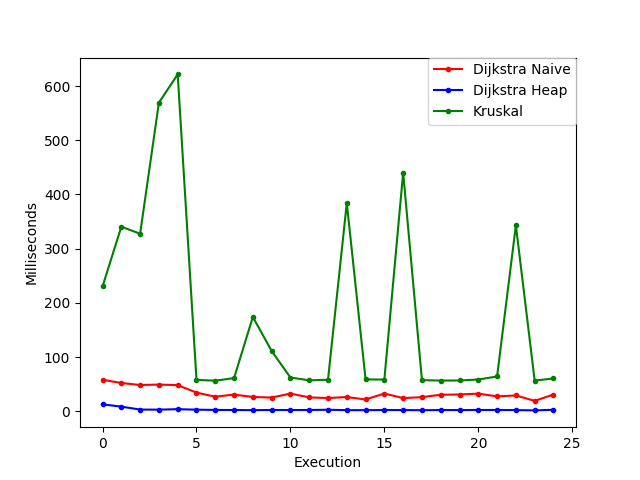
\includegraphics[width=.5\textwidth]{sparse}}
\subfloat[Graph with average degree of 20\%]{\label{fig:dense}
  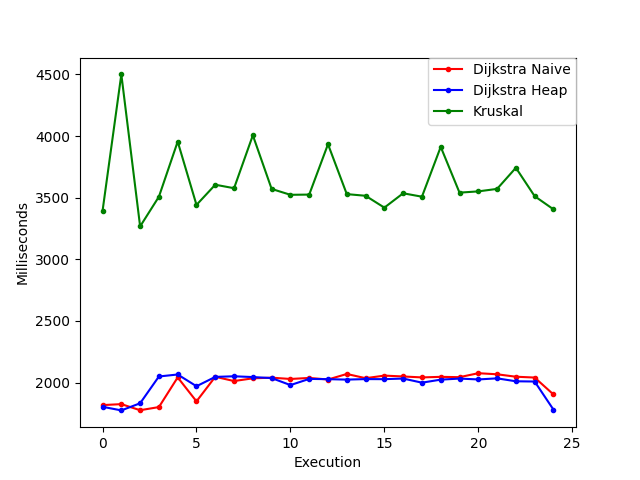
\includegraphics[width=.5\textwidth]{dense}}
\caption{Execution of the three algorithms on different vertex pairs}
\label{fig:execution_curves}
\end{figure}
\ \\

As expected the version of Dijkstra's algorithm that uses a heap to store the fringe vertices is always faster compared to the standard version on a sparse graph. Contrary to that, on a dense graph both performances are almost similar. Most of the times it performs slightly better but also sometimes worse than the standard version. Kruskal's algorithm performs much worse than both other algorithms on both graph versions. Also, its execution time varies much more than the time used for both other algorithms.
The standard version of Dijkstra's algorithm has an average runtime of 32.76 milliseconds on the sparse graph and 1992.30 milliseconds on the dense graph version.
The heap version of Dijkstra's algorithm in average runs in 3.29 milliseconds on the sparse and in 1989.29 milliseconds on the dense graph.
Kruskal's algorithm in average runs in 177.07 milliseconds on the sparse and in 3621.95 milliseconds on the dense graph.
This shows that with the current implementation Kruskal's algorithm takes 5.4 times longer than the naive implementation of Dijkstra's algorithm on sparse graphs. On the dense version it takes 1.8 times longer than the naive algorithm.

\section{Problems}
The difficulties implementing the project were mainly related to writing the code for the graph generation and the implementation of the max heap since it uses the three different arrays to store indices like the name, the position, and the value of the node. It became very confusing and debugging was therefore cumbersome. I first tried to debug using \textit{print} statements in the command line. Even with only 10 nodes stored in the heap it was already hard to see whether the changes made during execution led to intended results. I ended up using the debugger and fixed the heap data structure by following every single step writing down the state of the heap to track the operations.
The unit tests that I had written helped me a lot in the development process. Based on them I could be sure that whatever I would change with introducing new code, it would not break the already existing code. Unfortunately, there was an edge case for the graph generation that I did not test correctly but luckily another test that I wrote for the Kruskal's algorithm showed that I had made a mistake. While generating the graph random edges get added. I ended up adding the vertex $w$ to the LinkedList at position $v$ with its corresponding weight. But when adding the edge the other way around I put a different weight value in the edge. By testing that Kruskal's algorithm only operated on edges without duplicates I saw that I always got two edges with the same $v$ and $w$ but with different edge weights. This led to unpredictable behavior while running the Kruskal's algorithm because the removal of duplicate edges was not successful due of similar edges that had different weights. 
In contrast to that the implementation of the algorithms was successful from the start on.

\section{Further Improvements and Thoughts}
As described in the Implementation chapter, the project was implemented using Java. By using a lower level language like C++ or even C the performance of the algorithms could be further improved. 
The implementation makes use of the built-in \textit{ArrayList} data structure. This is an array wrapper that handles the memory allocation automatically. It therefore introduces some overhead to the code since every time an index is accessed an additional function call is made instead of just accessing an element directly by using an index. The same applies to the getter and setter functions of the Vertex object although this should not introduce much more computational time since the function call just returns a value. Due to the encapsulation principle that comes with Java or object-oriented programming in general this could but should not not be changed by making the object variables public.

To improve memory efficiency, the initialization of the heap in the Kruskal version should not use a maximum size of $n^2$ but rather the actual number of edges without any duplicates. Because in our case we have only a maximum number of 1000 edges per vertex we could set the maximum size to $2 * (1000 * n)$ or set it dynamically depending on the average degree of a vertex. Another way would be to iterate over the whole adjecency list and reading the exact number of edges – but this would add another operation of time $O(n)$.

When it comes to the implementation of Kruskal's algorithm I am not quite sure if my solution could be somehow improved. Although the algorithm itself works perfectly fine, which is proven by the written unit tests, I think that the runtime which is much longer than for both of the other algorithms is maybe not perfect. 
Due to the fact that my graphs are stored as an array of linked lists and every node in such a list is a Vertex object that only stores a name and a weight, the algorithm first has to build a list of Edge objects that store both vertices $v$ and $w$ in them. This is necessary because the operations on the disjoint set data structure need both vertex names that make up an edge. This step alone with the removal of duplicate edges takes $O(n^2)$ time, what makes the algorithm very slow. I think if one would not consider this step while measuring the time the algorithm could in fact perform better than the other two.

\newpage
\bibliographystyle{plain}	
\bibliography{literature}
\appendix

\section{Appendix}
The source code can be found in the \textit{src} directory. A corresponding executable \textbf{jar} file, built from the source code, is also included and can be found in the submitted folder.\\
To run the code JDK 11 or higher and the Java Runtime has to be installed on the machine.\\

To compile the code navigate into the root directory and run: \textbf{javac} \textit{./src/Main.java}\\

If compiled successfully, run the program with: \textbf{java} \textit{src/Main}\\

Alternatively run the executable \textbf{jar} file by typing: \textbf{java} -jar main.jar\\

The program will automatically write the results to the text file \textit{results.txt}.
\end{document}